% Options for packages loaded elsewhere
\PassOptionsToPackage{unicode}{hyperref}
\PassOptionsToPackage{hyphens}{url}
%
\documentclass[
  12pt,
]{article}
\usepackage{lmodern}
\usepackage{amssymb,amsmath}
\usepackage{ifxetex,ifluatex}
\ifnum 0\ifxetex 1\fi\ifluatex 1\fi=0 % if pdftex
  \usepackage[T1]{fontenc}
  \usepackage[utf8]{inputenc}
  \usepackage{textcomp} % provide euro and other symbols
\else % if luatex or xetex
  \usepackage{unicode-math}
  \defaultfontfeatures{Scale=MatchLowercase}
  \defaultfontfeatures[\rmfamily]{Ligatures=TeX,Scale=1}
\fi
% Use upquote if available, for straight quotes in verbatim environments
\IfFileExists{upquote.sty}{\usepackage{upquote}}{}
\IfFileExists{microtype.sty}{% use microtype if available
  \usepackage[]{microtype}
  \UseMicrotypeSet[protrusion]{basicmath} % disable protrusion for tt fonts
}{}
\makeatletter
\@ifundefined{KOMAClassName}{% if non-KOMA class
  \IfFileExists{parskip.sty}{%
    \usepackage{parskip}
  }{% else
    \setlength{\parindent}{0pt}
    \setlength{\parskip}{6pt plus 2pt minus 1pt}}
}{% if KOMA class
  \KOMAoptions{parskip=half}}
\makeatother
\usepackage{xcolor}
\IfFileExists{xurl.sty}{\usepackage{xurl}}{} % add URL line breaks if available
\IfFileExists{bookmark.sty}{\usepackage{bookmark}}{\usepackage{hyperref}}
\hypersetup{
  hidelinks,
  pdfcreator={LaTeX via pandoc}}
\urlstyle{same} % disable monospaced font for URLs
\usepackage[margin=1in]{geometry}
\usepackage{longtable,booktabs}
% Correct order of tables after \paragraph or \subparagraph
\usepackage{etoolbox}
\makeatletter
\patchcmd\longtable{\par}{\if@noskipsec\mbox{}\fi\par}{}{}
\makeatother
% Allow footnotes in longtable head/foot
\IfFileExists{footnotehyper.sty}{\usepackage{footnotehyper}}{\usepackage{footnote}}
\makesavenoteenv{longtable}
\usepackage{graphicx,grffile}
\makeatletter
\def\maxwidth{\ifdim\Gin@nat@width>\linewidth\linewidth\else\Gin@nat@width\fi}
\def\maxheight{\ifdim\Gin@nat@height>\textheight\textheight\else\Gin@nat@height\fi}
\makeatother
% Scale images if necessary, so that they will not overflow the page
% margins by default, and it is still possible to overwrite the defaults
% using explicit options in \includegraphics[width, height, ...]{}
\setkeys{Gin}{width=\maxwidth,height=\maxheight,keepaspectratio}
% Set default figure placement to htbp
\makeatletter
\def\fps@figure{htbp}
\makeatother
\setlength{\emergencystretch}{3em} % prevent overfull lines
\providecommand{\tightlist}{%
  \setlength{\itemsep}{0pt}\setlength{\parskip}{0pt}}
\setcounter{secnumdepth}{-\maxdimen} % remove section numbering
\usepackage{setspace}\doublespacing
\usepackage{float}
\usepackage{caption}
\usepackage{booktabs}
\usepackage{longtable}
\usepackage{array}
\usepackage{multirow}
\usepackage{wrapfig}
\usepackage{float}
\usepackage{colortbl}
\usepackage{pdflscape}
\usepackage{tabu}
\usepackage{threeparttable}
\usepackage{threeparttablex}
\usepackage[normalem]{ulem}
\usepackage{makecell}
\usepackage{xcolor}

\author{}
\date{\vspace{-2.5em}}

\begin{document}

\captionsetup[figure]{labelformat=empty}
\captionsetup[table]{labelformat=empty}
\renewcommand{\figurename}{}

\hypertarget{supporting-information}{%
\section{Supporting information:}\label{supporting-information}}

\hypertarget{recipient-and-donor-characteristics-govern-the-hierarchical-structure-of-heterospecific-pollen-competition-networks}{%
\section{Recipient and donor characteristics govern the hierarchical
structure of heterospecific pollen competition
networks}\label{recipient-and-donor-characteristics-govern-the-hierarchical-structure-of-heterospecific-pollen-competition-networks}}

\textbf{Authors:} Jose B. Lanuza, Ignasi Bartomeus, Tia-Lynn Ashman,
Romina Rader

The following Supporting Information is available for this article:

\textbf{Table S1.} Species names, common names, varieties and sources of
the different seeds.

\textbf{Table S2.} Numerical values of all the traits measured for each
species.

\textbf{Table S3.} Seed set in percentage for hand cross-pollination,
hand self-pollination, natural selfing and apomixis for all species.

\textbf{Table S4.} Estimates, standard error, t-value and P-value of the
effect of the different 9 donors on each recipient species.

\textbf{Table S5.} Number of seeds produced with 100\% foreign pollen
treatments for the different recipient species.

\textbf{Table S6.} Phylogenetic signal and significance for all the
different traits

\textbf{Table S7.} Procrustes analysis results.

\textbf{Figure S1}. Total amount of pollen deposited per stigma.

\textbf{Figure S2}. Pollen ratios for the different recipient species.

\textbf{Figure S3}. Pollen ratios for the different recipient species by
family.

\textbf{Figure S4}. Statistical comparison of the pollen ratios by
family.

\textbf{Figure S5}. Unipartite bidirectional network with asymmetrical
effect.

\textbf{Figure S6}. Correlation matrix for all the different traits.

\textbf{Figure S7}. Species reproductive biology.

\textbf{Figure S8}. Grouped effect sizes by family for each recipient
species.

\newpage

\begingroup\fontsize{7}{9}\selectfont

\begin{longtabu} to \linewidth {>{\raggedright}X>{\raggedright}X>{\raggedright}X>{\raggedright}X}
\caption{\label{tab:unnamed-chunk-1}\textbf{Table S1.} Species names, common names, varieties and sources of the different seeds.}\\
\toprule
\textbf{Species} & \textbf{Common\_names} & \textbf{Variety} & \textbf{Source}\\
\midrule
\endfirsthead
\caption[]{\textbf{Table S1.} Species names, common names, varieties and sources of the different seeds. \textit{(continued)}}\\
\toprule
Species & Common\_names & Variety & Source\\
\midrule
\endhead
\
\endfoot
\bottomrule
\endlastfoot
\rowcolor{gray!6}  Brassica oleracea & Wild cabbage & Capitata & https://www.mrfothergills.com.au/\\
\addlinespace
Brassica rapa & Pak choi & Chinensis & https://www.mrfothergills.com.au/\\
\addlinespace
\rowcolor{gray!6}  Eruca sativa & Rocket &  & https://www.mrfothergills.com.au/\\
\addlinespace
Sinapis alba & White mustard &  & https://www.mrfothergills.com.au/\\
\addlinespace
\rowcolor{gray!6}  Ipomoea aquatica & Water spinach &  & https://www.theseedcollection.com.au/\\
\addlinespace
Ipomoea purpurea & Morning glory &  & http://www.shaman-australis.com.au\\
\addlinespace
\rowcolor{gray!6}  Capsicum annuum & Capsicum & California Wonder & https://www.edenseeds.com.au\\
\addlinespace
Petunia integrifolia & Petunia &  & https://www.dianeseeds.com/\\
\addlinespace
\rowcolor{gray!6}  Solanum lycopersicum & Tomato & Tommy Toe & https://www.mrfothergills.com.au/\\
\addlinespace
Solanum melongena & Eggplant & Little Fingers & https://www.4seasonsseeds.com.au/\\*
\end{longtabu}
\endgroup{}

\begin{landscape}


\begin{table}

\caption{\label{tab:unnamed-chunk-2}\textbf{Table S2.} Measurements ($\bar{X}$ ± SD) for all the 13 different traits for all plant species.}
\centering
\resizebox{\linewidth}{!}{
\fontsize{6}{8}\selectfont
\begin{tabu} to \linewidth {>{\raggedright\arraybackslash}p{2cm}>{\raggedleft}X>{\raggedleft}X>{\raggedleft}X>{\raggedleft}X>{\raggedleft}X>{\raggedleft}X>{\raggedleft}X>{\raggedleft}X>{\raggedleft}X>{\raggedleft}X>{\raggedleft}X>{\raggedleft}X>{\raggedleft}X}
\toprule
\textbf{Species} & \textbf{Pollen size $\mu$m} & \textbf{Pollen grains per anther} & \textbf{Ovule number} & \textbf{Pollen:ovule ratio} & \textbf{Stigma area $\mu$m$^{2}$} & \textbf{Stigma length (mm)} & \textbf{Stigma width (mm)} & \textbf{Style length (mm)} & \textbf{Style width (mm)} & \textbf{Ovary length (mm)} & \textbf{Ovary width (mm)} & \textbf{Selfing rate} & \textbf{SI index}\\
\midrule
\rowcolor{gray!6}  Brassica oleracea & 27.72 & 42033 & 29 & 8696.48 & 0.62 & 0.53 & 0.88 & 2.32 & 0.65 & 5.93 & 1.11 & 0.0 & 0.00\\
\addlinespace
Brassica rapa & 25.35 & 7133 & 26 & 1646.08 & 0.36 & 0.37 & 0.73 & 1.08 & 0.52 & 3.53 & 0.88 & 0.0 & 0.00\\
\addlinespace
\rowcolor{gray!6}  Capsicum annuum & 32.46 & 30761 & 241 & 765.83 & 1.06 & 0.72 & 1.18 & 3.24 & 1.06 & 3.15 & 5.80 & 0.8 & 0.64\\
\addlinespace
Eruca versicaria & 24.95 & 22151 & 24 & 5537.75 & 0.35 & 0.73 & 0.67 & 6.60 & 0.73 & 4.42 & 0.94 & 0.1 & 0.02\\
\addlinespace
\rowcolor{gray!6}  Ipomoea aquatica & 70.10 & 858 & 4 & 1072.50 & 3.26 & 1.43 & 2.25 & 19.44 & 0.45 & 2.38 & 1.42 & 0.6 & 0.75\\
\addlinespace
Ipomoea purpurea & 97.59 & 654 & 6 & 545.00 & 2.27 & 1.24 & 1.88 & 28.23 & 0.58 & 1.06 & 1.57 & 1.0 & 2.74\\
\addlinespace
\rowcolor{gray!6}  Petunia integrifolia & 24.74 & 34657 & 220 & 787.66 & 1.17 & 0.80 & 1.32 & 14.65 & 0.45 & 3.13 & 1.77 & 0.9 & 0.26\\
\addlinespace
Sinapis alba & 33.59 & 3507 & 6 & 3507.00 & 0.55 & 0.63 & 0.91 & 3.62 & 0.77 & 1.98 & 1.07 & 0.7 & 1.12\\
\addlinespace
\rowcolor{gray!6}  Solanum lycopersicum & 22.00 & 28915 & 92 & 1885.76 & 0.09 & 0.19 & 0.35 & 6.47 & 0.31 & 1.16 & 1.13 & 0.7 & 0.48\\
\addlinespace
Solanum melongena & 25.18 & 166989 & 1010 & 992.01 & 1.14 & 0.96 & 1.33 & 11.33 & 0.94 & 4.02 & 3.55 & 1.0 & 1.45\\
\bottomrule
\end{tabu}}
\end{table}

\end{landscape}

\begin{longtable}[]{@{}lrrrr@{}}
\caption{\textbf{Table S3.} Seed:ovule ratio in percentage for hand
cross-pollination, hand self-pollination, spontaneous selfing and
apomixis for all species.}\tabularnewline
\toprule
\begin{minipage}[b]{0.19\columnwidth}\raggedright
Species\strut
\end{minipage} & \begin{minipage}[b]{0.21\columnwidth}\raggedleft
Hand cross-pollination\strut
\end{minipage} & \begin{minipage}[b]{0.20\columnwidth}\raggedleft
Hand self-pollination\strut
\end{minipage} & \begin{minipage}[b]{0.18\columnwidth}\raggedleft
Spontaneous selfing\strut
\end{minipage} & \begin{minipage}[b]{0.08\columnwidth}\raggedleft
Apomixis\strut
\end{minipage}\tabularnewline
\midrule
\endfirsthead
\toprule
\begin{minipage}[b]{0.19\columnwidth}\raggedright
Species\strut
\end{minipage} & \begin{minipage}[b]{0.21\columnwidth}\raggedleft
Hand cross-pollination\strut
\end{minipage} & \begin{minipage}[b]{0.20\columnwidth}\raggedleft
Hand self-pollination\strut
\end{minipage} & \begin{minipage}[b]{0.18\columnwidth}\raggedleft
Spontaneous selfing\strut
\end{minipage} & \begin{minipage}[b]{0.08\columnwidth}\raggedleft
Apomixis\strut
\end{minipage}\tabularnewline
\midrule
\endhead
\begin{minipage}[t]{0.19\columnwidth}\raggedright
Brassica oleracea\strut
\end{minipage} & \begin{minipage}[t]{0.21\columnwidth}\raggedleft
32.07\strut
\end{minipage} & \begin{minipage}[t]{0.20\columnwidth}\raggedleft
0.00\strut
\end{minipage} & \begin{minipage}[t]{0.18\columnwidth}\raggedleft
0.00\strut
\end{minipage} & \begin{minipage}[t]{0.08\columnwidth}\raggedleft
0\strut
\end{minipage}\tabularnewline
\begin{minipage}[t]{0.19\columnwidth}\raggedright
Brassica rapa\strut
\end{minipage} & \begin{minipage}[t]{0.21\columnwidth}\raggedleft
44.97\strut
\end{minipage} & \begin{minipage}[t]{0.20\columnwidth}\raggedleft
0.00\strut
\end{minipage} & \begin{minipage}[t]{0.18\columnwidth}\raggedleft
0.00\strut
\end{minipage} & \begin{minipage}[t]{0.08\columnwidth}\raggedleft
0\strut
\end{minipage}\tabularnewline
\begin{minipage}[t]{0.19\columnwidth}\raggedright
Capsicum annuum\strut
\end{minipage} & \begin{minipage}[t]{0.21\columnwidth}\raggedleft
80.00\strut
\end{minipage} & \begin{minipage}[t]{0.20\columnwidth}\raggedleft
56.47\strut
\end{minipage} & \begin{minipage}[t]{0.18\columnwidth}\raggedleft
19.34\strut
\end{minipage} & \begin{minipage}[t]{0.08\columnwidth}\raggedleft
0\strut
\end{minipage}\tabularnewline
\begin{minipage}[t]{0.19\columnwidth}\raggedright
Eruca sativa\strut
\end{minipage} & \begin{minipage}[t]{0.21\columnwidth}\raggedleft
23.75\strut
\end{minipage} & \begin{minipage}[t]{0.20\columnwidth}\raggedleft
0.42\strut
\end{minipage} & \begin{minipage}[t]{0.18\columnwidth}\raggedleft
0.00\strut
\end{minipage} & \begin{minipage}[t]{0.08\columnwidth}\raggedleft
0\strut
\end{minipage}\tabularnewline
\begin{minipage}[t]{0.19\columnwidth}\raggedright
Ipomoea aquatica\strut
\end{minipage} & \begin{minipage}[t]{0.21\columnwidth}\raggedleft
40.00\strut
\end{minipage} & \begin{minipage}[t]{0.20\columnwidth}\raggedleft
30.00\strut
\end{minipage} & \begin{minipage}[t]{0.18\columnwidth}\raggedleft
20.00\strut
\end{minipage} & \begin{minipage}[t]{0.08\columnwidth}\raggedleft
0\strut
\end{minipage}\tabularnewline
\begin{minipage}[t]{0.19\columnwidth}\raggedright
Ipomoea purpurea\strut
\end{minipage} & \begin{minipage}[t]{0.21\columnwidth}\raggedleft
31.67\strut
\end{minipage} & \begin{minipage}[t]{0.20\columnwidth}\raggedleft
86.67\strut
\end{minipage} & \begin{minipage}[t]{0.18\columnwidth}\raggedleft
31.67\strut
\end{minipage} & \begin{minipage}[t]{0.08\columnwidth}\raggedleft
0\strut
\end{minipage}\tabularnewline
\begin{minipage}[t]{0.19\columnwidth}\raggedright
Petunia integrifolia\strut
\end{minipage} & \begin{minipage}[t]{0.21\columnwidth}\raggedleft
80.16\strut
\end{minipage} & \begin{minipage}[t]{0.20\columnwidth}\raggedleft
24.77\strut
\end{minipage} & \begin{minipage}[t]{0.18\columnwidth}\raggedleft
0.00\strut
\end{minipage} & \begin{minipage}[t]{0.08\columnwidth}\raggedleft
0\strut
\end{minipage}\tabularnewline
\begin{minipage}[t]{0.19\columnwidth}\raggedright
Sinapis alba\strut
\end{minipage} & \begin{minipage}[t]{0.21\columnwidth}\raggedleft
41.67\strut
\end{minipage} & \begin{minipage}[t]{0.20\columnwidth}\raggedleft
48.33\strut
\end{minipage} & \begin{minipage}[t]{0.18\columnwidth}\raggedleft
5.00\strut
\end{minipage} & \begin{minipage}[t]{0.08\columnwidth}\raggedleft
15\strut
\end{minipage}\tabularnewline
\begin{minipage}[t]{0.19\columnwidth}\raggedright
Solanum lycopersium\strut
\end{minipage} & \begin{minipage}[t]{0.21\columnwidth}\raggedleft
85.65\strut
\end{minipage} & \begin{minipage}[t]{0.20\columnwidth}\raggedleft
41.20\strut
\end{minipage} & \begin{minipage}[t]{0.18\columnwidth}\raggedleft
68.48\strut
\end{minipage} & \begin{minipage}[t]{0.08\columnwidth}\raggedleft
0\strut
\end{minipage}\tabularnewline
\begin{minipage}[t]{0.19\columnwidth}\raggedright
Solanum melongena\strut
\end{minipage} & \begin{minipage}[t]{0.21\columnwidth}\raggedleft
60.48\strut
\end{minipage} & \begin{minipage}[t]{0.20\columnwidth}\raggedleft
74.87\strut
\end{minipage} & \begin{minipage}[t]{0.18\columnwidth}\raggedleft
21.56\strut
\end{minipage} & \begin{minipage}[t]{0.08\columnwidth}\raggedleft
0\strut
\end{minipage}\tabularnewline
\bottomrule
\end{longtable}

\newpage

\begin{landscape}


\begin{table}

\caption{\label{tab:unnamed-chunk-4}\textbf{Table S4.} Species x species matrix with the significance of effect “yes” or “no” of the different donors on seed set from the linear mixed effect models. The category of “yes” represents significant effect of the donors (columns) on the different recipient species (rows) and “no” lack of significant reduction of seed set from the control. Significance was tested for all species by comparing with a control of hand cross-pollination with conspecific pollen.}
\centering
\resizebox{\linewidth}{!}{
\fontsize{6}{8}\selectfont
\begin{tabu} to \linewidth {>{\raggedright\arraybackslash}p{2cm}>{\raggedright}X>{\raggedright}X>{\raggedright}X>{\raggedright}X>{\raggedright}X>{\raggedright}X>{\raggedright}X>{\raggedright}X>{\raggedright}X>{\raggedright}X>{\raggedleft}X>{\raggedleft}X}
\toprule
\textbf{X} & \textbf{B..oleracea} & \textbf{B..rapa} & \textbf{E..sativa} & \textbf{S..alba} & \textbf{I..aquatica} & \textbf{I..purpurea} & \textbf{C..annuum} & \textbf{P..integrifolia} & \textbf{S..lycopersicum} & \textbf{S..melongena} & \textbf{S.Significant.effect.of.donors} & \textbf{X..donors.with.significant.effect}\\
\midrule
\rowcolor{gray!6}  B. oleracea &  & Yes & Yes & Yes & Yes & Yes & Yes & Yes & Yes & Yes & 9 & 100.0\\
\addlinespace
B. rapa & No &  & Yes & Yes & Yes & Yes & Yes & Yes & Yes & Yes & 8 & 88.9\\
\addlinespace
\rowcolor{gray!6}  E. sativa & Yes & No &  & No & Yes & No & No & No & No & No & 1 & 22.2\\
\addlinespace
S. alba & No & Yes & No &  & Yes & Yes & Yes & No & No & No & 4 & 44.4\\
\addlinespace
\rowcolor{gray!6}  I. aquatica & Yes & Yes & Yes & Yes &  & Yes & Yes & Yes & Yes & Yes & 9 & 100.0\\
\addlinespace
I. purpurea & No & No & Yes & No & No &  & Yes & No & Yes & No & 3 & 33.3\\
\addlinespace
\rowcolor{gray!6}  C. annuum & Yes & Yes & No & Yes & No & Yes &  & Yes & Yes1 & Yes & 7 & 77.8\\
\addlinespace
P. integrifolia & Yes & No & No & Yes & Yes & Yes & No &  & Yes & Yes & 6 & 67.7\\
\addlinespace
\rowcolor{gray!6}  S. lycopersicum & No & Yes & Yes & Yes & Yes & Yes & Yes & Yes &  & Yes & 8 & 88.9\\
\addlinespace
S. melongena & No & Yes & Yes & No & Yes & Yes & Yes & No & No &  & 5 & 55.6\\
\addlinespace
\rowcolor{gray!6}   &  &  &  &  &  &  &  &  &  &  & 60 & 66.7\\
\bottomrule
\end{tabu}}
\end{table}

\end{landscape}

\begin{longtable}[]{@{}lrrrr@{}}
\caption{\textbf{Table S5.} Output of linear models of the effect of the
different donors on the seed set of each recipient
species.}\tabularnewline
\toprule
& Est. & S.E. & t val. & p\tabularnewline
\midrule
\endfirsthead
\toprule
& Est. & S.E. & t val. & p\tabularnewline
\midrule
\endhead
Petunia integrifolia - (Intercept) & 4.63 & 0.49 & 9.36 &
0.00\tabularnewline
Petunia integrifolia - Brassica oleracea & -1.84 & 0.81 & -2.27 &
0.03\tabularnewline
Petunia integrifolia - Brassica rapa & -0.97 & 0.81 & -1.19 &
0.24\tabularnewline
Petunia integrifolia - Capsicum annuum & 0.78 & 0.81 & 0.96 &
0.34\tabularnewline
Petunia integrifolia - Eruca vesicaria & -0.91 & 0.81 & -1.12 &
0.26\tabularnewline
Petunia integrifolia - Ipomoea aquatica & -3.18 & 0.81 & -3.92 &
0.00\tabularnewline
Petunia integrifolia - Ipomoea purpurea & -4.21 & 0.81 & -5.19 &
0.00\tabularnewline
Petunia integrifolia - Sinapis alba & -2.99 & 0.81 & -3.69 &
0.00\tabularnewline
Petunia integrifolia - Solanum lycopersicum & -2.40 & 0.81 & -2.96 &
0.00\tabularnewline
Petunia integrifolia - Solanum melongena & -2.66 & 0.81 & -3.27 &
0.00\tabularnewline
Solanum lycopersicum - (Intercept) & 4.39 & 0.24 & 18.54 &
0.00\tabularnewline
Solanum lycopersicum - Brassica oleracea & -0.47 & 0.41 & -1.14 &
0.26\tabularnewline
Solanum lycopersicum - Brassica rapa & -2.74 & 0.41 & -6.67 &
0.00\tabularnewline
Solanum lycopersicum - Capsicum annuum & -4.39 & 0.41 & -10.71 &
0.00\tabularnewline
Solanum lycopersicum - Eruca vesicaria & -2.97 & 0.41 & -7.25 &
0.00\tabularnewline
Solanum lycopersicum - Ipomoea aquatica & -4.13 & 0.41 & -10.06 &
0.00\tabularnewline
Solanum lycopersicum - Ipomoea purpurea & -3.80 & 0.41 & -9.27 &
0.00\tabularnewline
Solanum lycopersicum - Petunia integrifolia & -1.82 & 0.41 & -4.44 &
0.00\tabularnewline
Solanum lycopersicum - Sinapis alba & -3.72 & 0.41 & -9.08 &
0.00\tabularnewline
Solanum lycopersicum - Solanum melongena & -1.84 & 0.41 & -4.49 &
0.00\tabularnewline
Solanum melongena - (Intercept) & 6.34 & 0.70 & 9.09 &
0.00\tabularnewline
Solanum melongena - Brassica oleracea & -0.67 & 0.99 & -0.68 &
0.50\tabularnewline
Solanum melongena - Brassica rapa & -4.33 & 0.99 & -4.39 &
0.00\tabularnewline
Solanum melongena - Capsicum annuum & -2.33 & 0.99 & -2.36 &
0.02\tabularnewline
Solanum melongena - Eruca vesicaria & -3.12 & 0.99 & -3.16 &
0.00\tabularnewline
Solanum melongena - Ipomoea aquatica & -6.34 & 0.99 & -6.43 &
0.00\tabularnewline
Solanum melongena - Ipomoea purpurea & -2.71 & 0.99 & -2.74 &
0.01\tabularnewline
Solanum melongena - Petunia integrifolia & -1.43 & 0.99 & -1.45 &
0.15\tabularnewline
Solanum melongena - Sinapis alba & -1.11 & 0.99 & -1.12 &
0.26\tabularnewline
Solanum melongena - Solanum lycopersicum & -0.84 & 0.99 & -0.86 &
0.39\tabularnewline
Capsicum annuum - (Intercept) & 4.59 & 0.52 & 8.78 & 0.00\tabularnewline
Capsicum annuum - Brassica oleracea & -1.80 & 0.74 & -2.43 &
0.02\tabularnewline
Capsicum annuum - Brassica rapa & -2.51 & 0.74 & -3.39 &
0.00\tabularnewline
Capsicum annuum - Eruca vesicaria & -0.63 & 0.74 & -0.85 &
0.40\tabularnewline
Capsicum annuum - Ipomoea aquatica & -1.36 & 0.74 & -1.84 &
0.07\tabularnewline
Capsicum annuum - Ipomoea purpurea & -4.00 & 0.74 & -5.41 &
0.00\tabularnewline
Capsicum annuum - Petunia integrifolia & -4.59 & 0.74 & -6.21 &
0.00\tabularnewline
Capsicum annuum - Sinapis alba & -3.63 & 0.74 & -4.92 &
0.00\tabularnewline
Capsicum annuum - Solanum lycopersicum & -1.52 & 0.74 & -2.06 &
0.04\tabularnewline
Capsicum annuum - Solanum melongena & -3.29 & 0.74 & -4.46 &
0.00\tabularnewline
Brassica oleracea - (Intercept) & 1.99 & 0.22 & 8.98 &
0.00\tabularnewline
Brassica oleracea - Brassica rapa & -1.37 & 0.31 & -4.35 &
0.00\tabularnewline
Brassica oleracea - Capsicum annuum & -0.87 & 0.31 & -2.76 &
0.01\tabularnewline
Brassica oleracea - Eruca vesicaria & -1.92 & 0.31 & -6.13 &
0.00\tabularnewline
Brassica oleracea - Ipomoea aquatica & -1.91 & 0.27 & -7.04 &
0.00\tabularnewline
Brassica oleracea - Ipomoea purpurea & -1.99 & 0.31 & -6.35 &
0.00\tabularnewline
Brassica oleracea - Petunia integrifolia & -1.64 & 0.31 & -5.21 &
0.00\tabularnewline
Brassica oleracea - Sinapis alba & -1.57 & 0.31 & -4.99 &
0.00\tabularnewline
Brassica oleracea - Solanum lycopersicum & -1.47 & 0.31 & -4.70 &
0.00\tabularnewline
Brassica oleracea - Solanum melongena & -1.61 & 0.31 & -5.12 &
0.00\tabularnewline
Brassica rapa - (Intercept) & 2.37 & 0.19 & 12.49 & 0.00\tabularnewline
Brassica rapa - Brassica oleracea & -0.54 & 0.29 & -1.89 &
0.06\tabularnewline
Brassica rapa - Capsicum annuum & -1.42 & 0.29 & -4.94 &
0.00\tabularnewline
Brassica rapa - Eruca vesicaria & -2.37 & 0.29 & -8.24 &
0.00\tabularnewline
Brassica rapa - Ipomoea aquatica & -1.92 & 0.29 & -6.67 &
0.00\tabularnewline
Brassica rapa - Ipomoea purpurea & -2.26 & 0.29 & -7.86 &
0.00\tabularnewline
Brassica rapa - Petunia integrifolia & -2.37 & 0.29 & -8.24 &
0.00\tabularnewline
Brassica rapa - Sinapis alba & -2.37 & 0.29 & -8.24 &
0.00\tabularnewline
Brassica rapa - Solanum lycopersicum & -1.88 & 0.29 & -6.55 &
0.00\tabularnewline
Brassica rapa - Solanum melongena & -2.37 & 0.29 & -8.24 &
0.00\tabularnewline
Eruca sativa - (Intercept) & 1.34 & 0.35 & 3.80 & 0.00\tabularnewline
Eruca sativa - Brassica oleracea & -1.34 & 0.50 & -2.69 &
0.01\tabularnewline
Eruca sativa - Brassica rapa & 0.66 & 0.50 & 1.32 & 0.19\tabularnewline
Eruca sativa - Capsicum annuum & -0.27 & 0.50 & -0.55 &
0.58\tabularnewline
Eruca sativa - Ipomoea aquatica & 0.87 & 0.50 & 1.75 &
0.08\tabularnewline
Eruca sativa - Ipomoea purpurea & -0.19 & 0.50 & -0.39 &
0.70\tabularnewline
Eruca sativa - Petunia integrifolia & 0.20 & 0.50 & 0.41 &
0.68\tabularnewline
Eruca sativa - Sinapis alba & 0.32 & 0.50 & 0.65 & 0.52\tabularnewline
Eruca sativa - Solanum lycopersicum & -0.52 & 0.50 & -1.04 &
0.30\tabularnewline
Eruca sativa - Solanum melongena & 0.54 & 0.50 & 1.09 &
0.28\tabularnewline
Ipomoea purpurea - (Intercept) & 0.82 & 0.20 & 4.05 &
0.00\tabularnewline
Ipomoea purpurea - Brassica oleracea & 0.37 & 0.29 & 1.31 &
0.19\tabularnewline
Ipomoea purpurea - Brassica rapa & -0.41 & 0.29 & -1.43 &
0.16\tabularnewline
Ipomoea purpurea - Capsicum annuum & -0.82 & 0.29 & -2.86 &
0.01\tabularnewline
Ipomoea purpurea - Eruca vesicaria & -0.75 & 0.29 & -2.62 &
0.01\tabularnewline
Ipomoea purpurea - Ipomoea aquatica & 0.41 & 0.29 & 1.44 &
0.15\tabularnewline
Ipomoea purpurea - Petunia integrifolia & -0.37 & 0.29 & -1.31 &
0.19\tabularnewline
Ipomoea purpurea - Sinapis alba & -0.33 & 0.29 & -1.14 &
0.26\tabularnewline
Ipomoea purpurea - Solanum lycopersicum & -0.82 & 0.29 & -2.86 &
0.01\tabularnewline
Ipomoea purpurea - Solanum melongena & -0.24 & 0.29 & -0.82 &
0.41\tabularnewline
Ipomoea aquatica - (Intercept) & 0.80 & 0.09 & 9.36 &
0.00\tabularnewline
Ipomoea aquatica - Brassica oleracea & -0.80 & 0.12 & -6.62 &
0.00\tabularnewline
Ipomoea aquatica - Brassica rapa & -0.80 & 0.12 & -6.62 &
0.00\tabularnewline
Ipomoea aquatica - Capsicum annuum & -0.80 & 0.12 & -6.62 &
0.00\tabularnewline
Ipomoea aquatica - Eruca vesicaria & -0.80 & 0.12 & -6.62 &
0.00\tabularnewline
Ipomoea aquatica - Ipomoea purpurea & -0.80 & 0.12 & -6.62 &
0.00\tabularnewline
Ipomoea aquatica - Petunia integrifolia & -0.59 & 0.12 & -4.89 &
0.00\tabularnewline
Ipomoea aquatica - Sinapis alba & -0.80 & 0.12 & -6.62 &
0.00\tabularnewline
Ipomoea aquatica - Solanum lycopersicum & -0.69 & 0.12 & -5.70 &
0.00\tabularnewline
Ipomoea aquatica - Solanum melongena & -0.80 & 0.12 & -6.62 &
0.00\tabularnewline
\bottomrule
\end{longtable}

\newpage

\begin{longtable}[]{@{}llr@{}}
\caption{\textbf{Table S6.} Number of seeds produced with 100\% foreign
pollen (N=900). From 900 pollination events we found seed production in
just 13 specific cases and 0 seed production in the other 887
pollination events. In this table we show just the treatments that lead
to seed production.}\tabularnewline
\toprule
Recipient & Donor (100\% foreign pollen) & Seed number\tabularnewline
\midrule
\endfirsthead
\toprule
Recipient & Donor (100\% foreign pollen) & Seed number\tabularnewline
\midrule
\endhead
Solnamum lycopersicum & Sinapis alba & 3\tabularnewline
Solnamum melongena & Petunia integrifolia & 36\tabularnewline
Capsicum annuum & Eruca sativa & 3\tabularnewline
Capsicum annuum & Sinapis alba & 127\tabularnewline
Brassica rapa & Brassica oleracea & 2\tabularnewline
Brassica rapa & Brassica oleracea & 13\tabularnewline
Sinapis alba & Brassica oleracea & 7\tabularnewline
Sinapis alba & Brassica oleracea & 5\tabularnewline
Sinapis alba & Brassica oleracea & 7\tabularnewline
Sinapis alba & Capsicum annuum & 1\tabularnewline
Sinapis alba & Capsicum annuum & 6\tabularnewline
Sinapis alba & Solanum lycopersicum & 1\tabularnewline
Eruca sativa & Petunia integrifolia & 2\tabularnewline
\bottomrule
\end{longtable}

\newpage

\begin{longtable}[]{@{}rrl@{}}
\caption{\textbf{Table S7.} Phylogenetic signal and significance for all
the different traits.}\tabularnewline
\toprule
Lambda & \emph{P}-value & Traits\tabularnewline
\midrule
\endfirsthead
\toprule
Lambda & \emph{P}-value & Traits\tabularnewline
\midrule
\endhead
0.95 & 0.20 & Selfing rate\tabularnewline
1.00 & 0.00 & \textbf{Pollen size}\tabularnewline
0.00 & 1.00 & Pollen anther\tabularnewline
0.00 & 1.00 & Ovule number\tabularnewline
0.00 & 1.00 & Pollen-ovule ratio\tabularnewline
0.89 & 0.01 & \textbf{Stigmatic area}\tabularnewline
0.70 & 0.05 & Stigma length\tabularnewline
0.77 & 0.03 & \textbf{Stigma width}\tabularnewline
0.93 & 0.01 & \textbf{Style length}\tabularnewline
0.00 & 1.00 & Style width\tabularnewline
0.47 & 0.30 & Ovary length\tabularnewline
0.00 & 1.00 & Ovary width\tabularnewline
0.00 & 0.02 & \textbf{SI index}\tabularnewline
\bottomrule
\end{longtable}

\newpage

\begin{longtable}[]{@{}rrrll@{}}
\caption{\textbf{Table S8.} Procrustes correlation, sum of squares and
significance from Procrustes analysis between the matrix of effect sizes
(species x species matrix) and the distance matrix of each trait for all
families, just Solanaceae and just Brassicaceae.}\tabularnewline
\toprule
Correlation (r) & Sum of squares & \emph{P}-value & Traits &
Family\tabularnewline
\midrule
\endfirsthead
\toprule
Correlation (r) & Sum of squares & \emph{P}-value & Traits &
Family\tabularnewline
\midrule
\endhead
0.34 & 0.88 & 0.70 & Selfing rate & All\tabularnewline
0.36 & 0.87 & 0.42 & Pollen size & All\tabularnewline
0.35 & 0.88 & 0.57 & Pollen per anther & All\tabularnewline
0.33 & 0.89 & 0.55 & Number of ovules & All\tabularnewline
0.30 & 0.91 & 0.86 & Pollen-ovule ratio & All\tabularnewline
0.37 & 0.86 & 0.68 & Stigmatic area & All\tabularnewline
0.62 & 0.62 & 0.10 & Stigma length & All\tabularnewline
0.46 & 0.79 & 0.47 & Stigma width & All\tabularnewline
0.43 & 0.82 & 0.45 & Style length & All\tabularnewline
0.59 & 0.65 & 0.11 & Style width & All\tabularnewline
0.34 & 0.88 & 0.57 & Ovary length & All\tabularnewline
0.35 & 0.88 & 0.93 & Ovary width & All\tabularnewline
0.49 & 0.76 & 0.24 & Self-incompatibility index & All\tabularnewline
0.86 & 0.26 & 0.25 & Selfing rate & Solanaceae\tabularnewline
0.76 & 0.42 & 0.33 & Pollen size & Solanaceae\tabularnewline
0.42 & 0.82 & 0.79 & Pollen per anther & Solanaceae\tabularnewline
0.52 & 0.73 & 0.83 & Number of ovules & Solanaceae\tabularnewline
0.87 & 0.25 & 0.04 & Pollen-ovule ratio & Solanaceae\tabularnewline
0.82 & 0.33 & 0.17 & Stigmatic area & Solanaceae\tabularnewline
0.89 & 0.20 & 0.08 & Stigma length & Solanaceae\tabularnewline
0.84 & 0.29 & 0.12 & Stigma width & Solanaceae\tabularnewline
0.78 & 0.39 & 0.50 & Style length & Solanaceae\tabularnewline
0.52 & 0.73 & 0.71 & Style width & Solanaceae\tabularnewline
0.64 & 0.60 & 0.79 & Ovary length & Solanaceae\tabularnewline
0.87 & 0.23 & 0.17 & Ovary width & Solanaceae\tabularnewline
0.50 & 0.75 & 1.00 & Self-incompatibility index &
Solanaceae\tabularnewline
0.61 & 0.63 & 0.50 & Selfing rate & Brassicaceae\tabularnewline
0.60 & 0.64 & 0.71 & Pollen size & Brassicaceae\tabularnewline
0.40 & 0.84 & 0.96 & Pollen per anther & Brassicaceae\tabularnewline
0.62 & 0.61 & 0.42 & Number of ovules & Brassicaceae\tabularnewline
0.49 & 0.76 & 0.96 & Pollen-ovule ratio & Brassicaceae\tabularnewline
0.55 & 0.70 & 0.58 & Stigmatic area & Brassicaceae\tabularnewline
0.92 & 0.15 & 0.08 & Stigma length & Brassicaceae\tabularnewline
0.63 & 0.60 & 0.38 & Stigma width & Brassicaceae\tabularnewline
0.83 & 0.31 & 0.08 & Style length & Brassicaceae\tabularnewline
0.79 & 0.37 & 0.33 & Style width & Brassicaceae\tabularnewline
0.59 & 0.65 & 0.50 & Ovary length & Brassicaceae\tabularnewline
0.54 & 0.70 & 1.00 & Ovary width & Brassicaceae\tabularnewline
0.50 & 0.75 & 0.83 & Self-incompatibility index &
Brassicaceae\tabularnewline
\bottomrule
\end{longtable}

\newpage

\begin{figure}
\centering
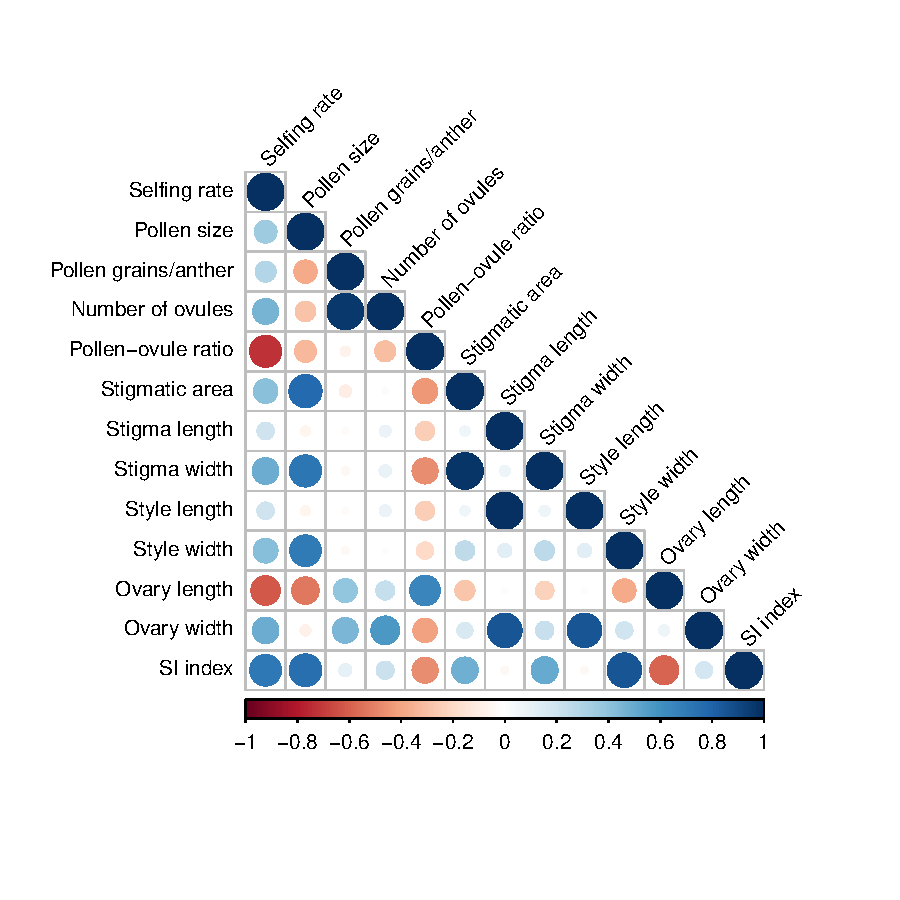
\includegraphics{Supp_Material_files/figure-latex/unnamed-chunk-9-1.pdf}
\caption{\textbf{Fig. S1} Average number of pollen grains per stigma for
20 different treatments (3 replicates per tratment). For each treatment,
we show the average number of conspecific pollen grains (grey) and
heterospecific pollen grains (light blue) per stigma. For each pair of
species on the x-axis, the first species is the recipient species, and
the second, the donor species.}
\end{figure}

\clearpage

\begin{figure}
\centering
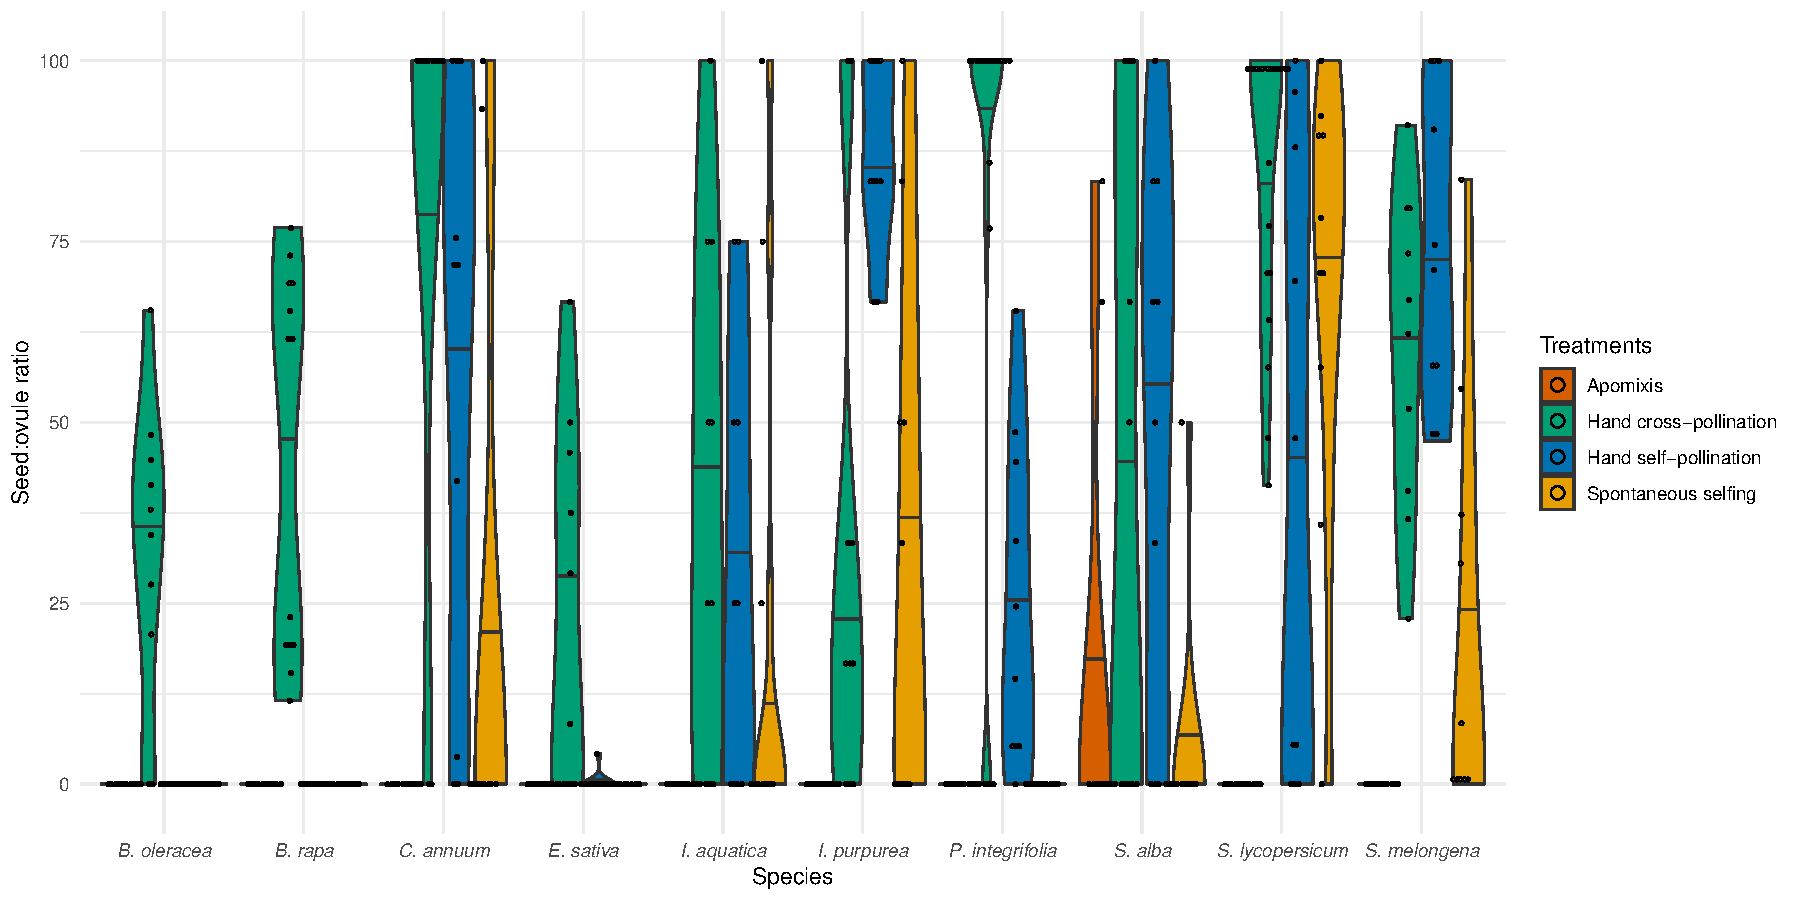
\includegraphics{Supp_Material_files/figure-latex/unnamed-chunk-10-1.pdf}
\caption{\textbf{Fig. S2} Average proportion of conspecific and
heterospecific pollen per stigma grouped by family, A) Brassicaceae, B)
Solanaceae and C) Convolvulaceae. These proportions (\%) are the number
of conspecific pollen grains or heterospecific pollen grains divided by
the total number of pollen grains per stigma for 20 different
treatments. We conducted 3 count replicates per treatment and then we
calculated the average number of pollen grains for these treatments. The
proportion of conspecific and heterospecific pollen are shown in grey
and light blue respectively. For each pair of species on the y-axis, the
first species is the pollen recipient and the second the pollen donor.
The vertical black line represents 50\% pollen of both donor and
recipient.}
\end{figure}

\clearpage

\begin{figure}
\centering
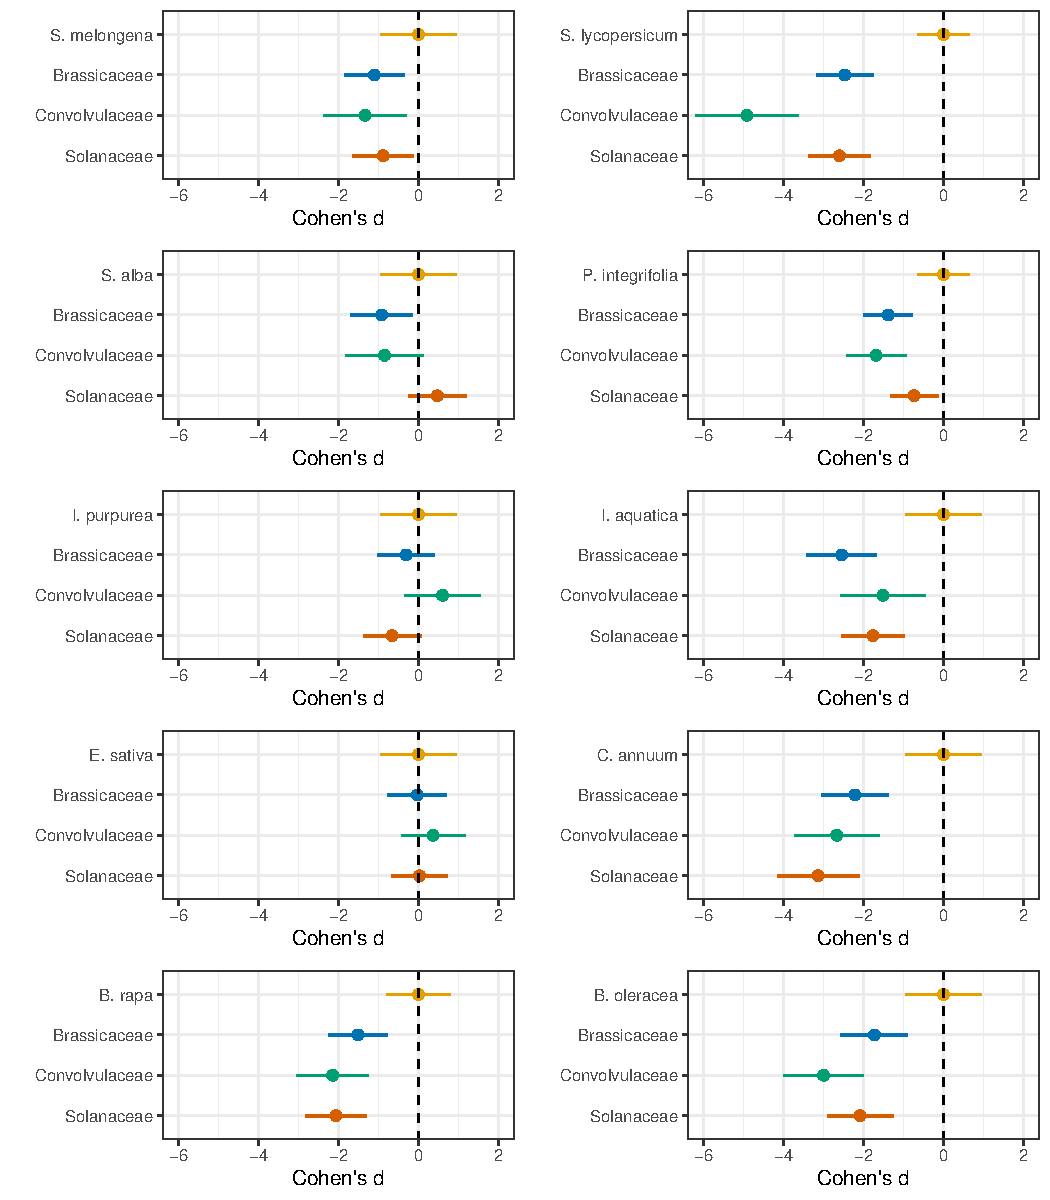
\includegraphics{Supp_Material_files/figure-latex/unnamed-chunk-11-1.pdf}
\caption{\textbf{Fig. S3} Average proportion (\%) of heterospecific and
conspecific pollen per family for the different 20 treatments counted.
We conducted 3 count replicates per treatment and then we calculated the
average number of pollen grains for these different 20 treatments.
Finally, we grouped by family these treatments in order to see general
tendencies across families as pollen donor and as pollen recipient.
Pollen ratios were considered as the number of conspecific or
heterospecific pollen grains divided by the total number of pollen
grains per stigma. On the y-axis, the first family on each pair of plant
families is the recipient one, and the second, the family of the donor.
The vertical bar on intercept 50, represents equal proportions of both
recipient (grey) and donor (light blue) pollen.}
\end{figure}

\clearpage

\begin{figure}
\centering
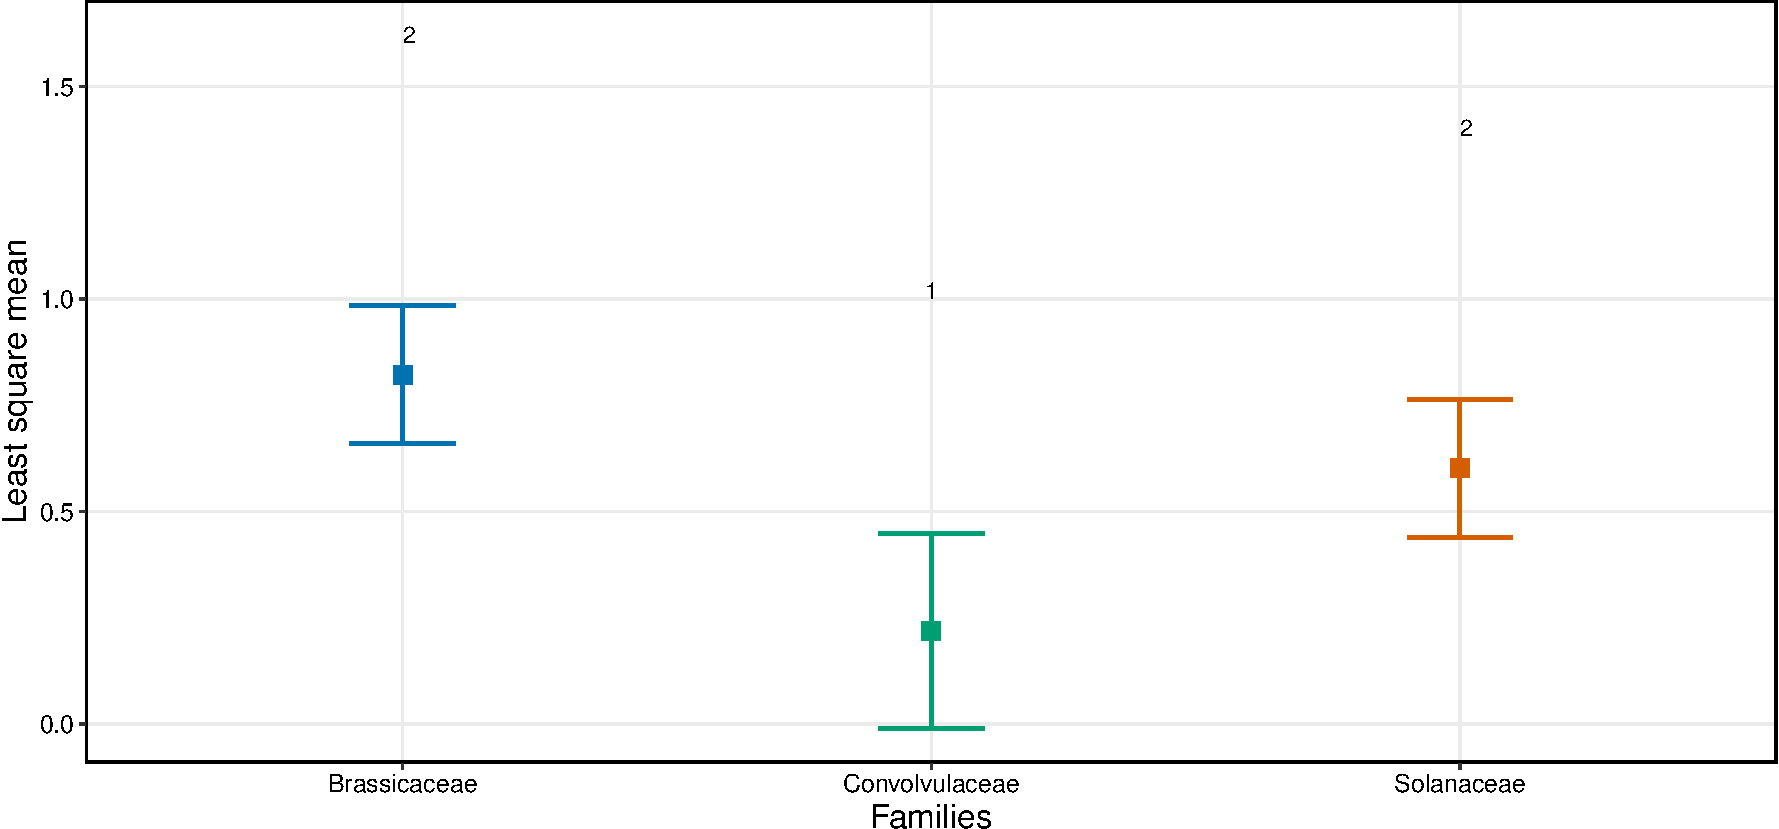
\includegraphics{Supp_Material_files/figure-latex/unnamed-chunk-12-1.pdf}
\caption{\textbf{Fig. S4} Pollen ratios comparisons between the
different pollen recipient families where the boxes represent least
square means, the error bars, confidence intervals 95\%, and sharing
numbers indicate no significant differences between groups (Tukey
adjusted comparisons). These pollen ratios (\%) are the total number of
heterospecific pollen grains divided by the total quantity of pollen
(conspecific pollen + heterospecific pollen), and then compared by
family (N=20). Brassicacea family is coloured in blue, Convolvulaceae in
green and Solanaceae in orange.}
\end{figure}

\newpage

\begin{figure}
\centering
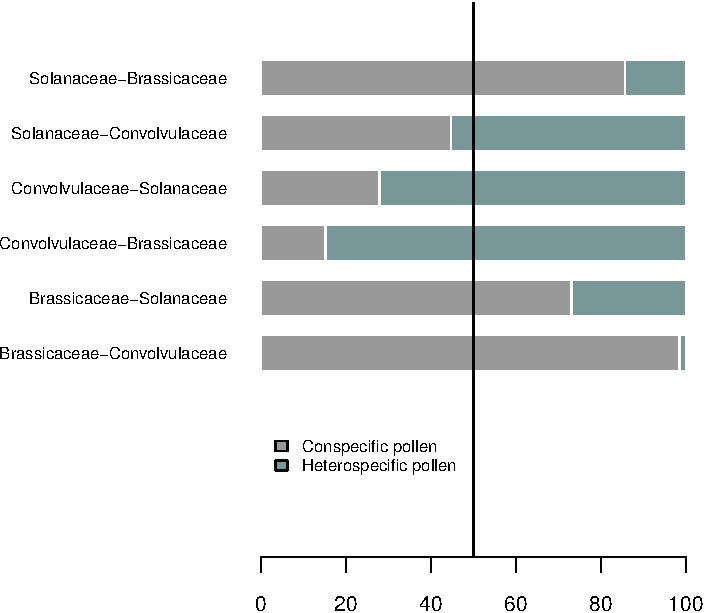
\includegraphics{Supp_Material_files/figure-latex/unnamed-chunk-13-1.pdf}
\caption{\textbf{Fig. S5} Unipartite bidirectional network with
asymmetrical effect. The lines with the arrow heads connect the impact
of foreign pollen (effect size) of each pollen donor species on each
recipient species. All the arrow heads point to the recipient species of
the reciprocal interaction. Lines of species that did not have a
negative impact are not represented. The different nodes and the effect
of the donor species on the recipient species appear coloured by family:
Solanaceae (orange), Brassicaceae (blue) and Convolvulaceae (green). The
intensity of the effect is represented by the line´s size where a larger
effect size corresponds to a thicker line and a thinner line to a
smaller effect size. Species code: BROL: Brassica oleracea, BRRA:
Brassica rapa, ERSA: Eruca sativa, SIAL: Sinapis alba, IPAQ: Ipomoea
aquatica, IPPU: Ipomoea purpurea, CAAN: Capsicum annuum, PEIN: Petunia
integrifolia, SOLY: Solanum lycopersicum, SOME: Solanum melongena.}
\end{figure}

\clearpage

\begin{figure}
\centering
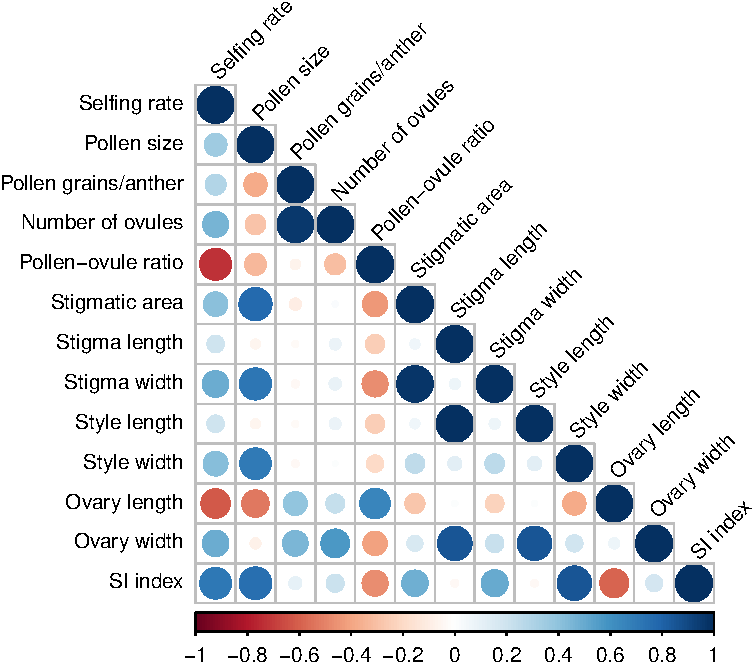
\includegraphics{Supp_Material_files/figure-latex/unnamed-chunk-14-1.pdf}
\caption{\textbf{Fig. S6} Graphical representation of the correlation
matrix of the different reproductive traits considered in the
experiment. Positive correlations are displayed in blue and negative in
red. The intensity, size and colour of the circles are proportional to
the correlation coefficient from Pearson's r.}
\end{figure}

\clearpage

\begin{figure}
\centering
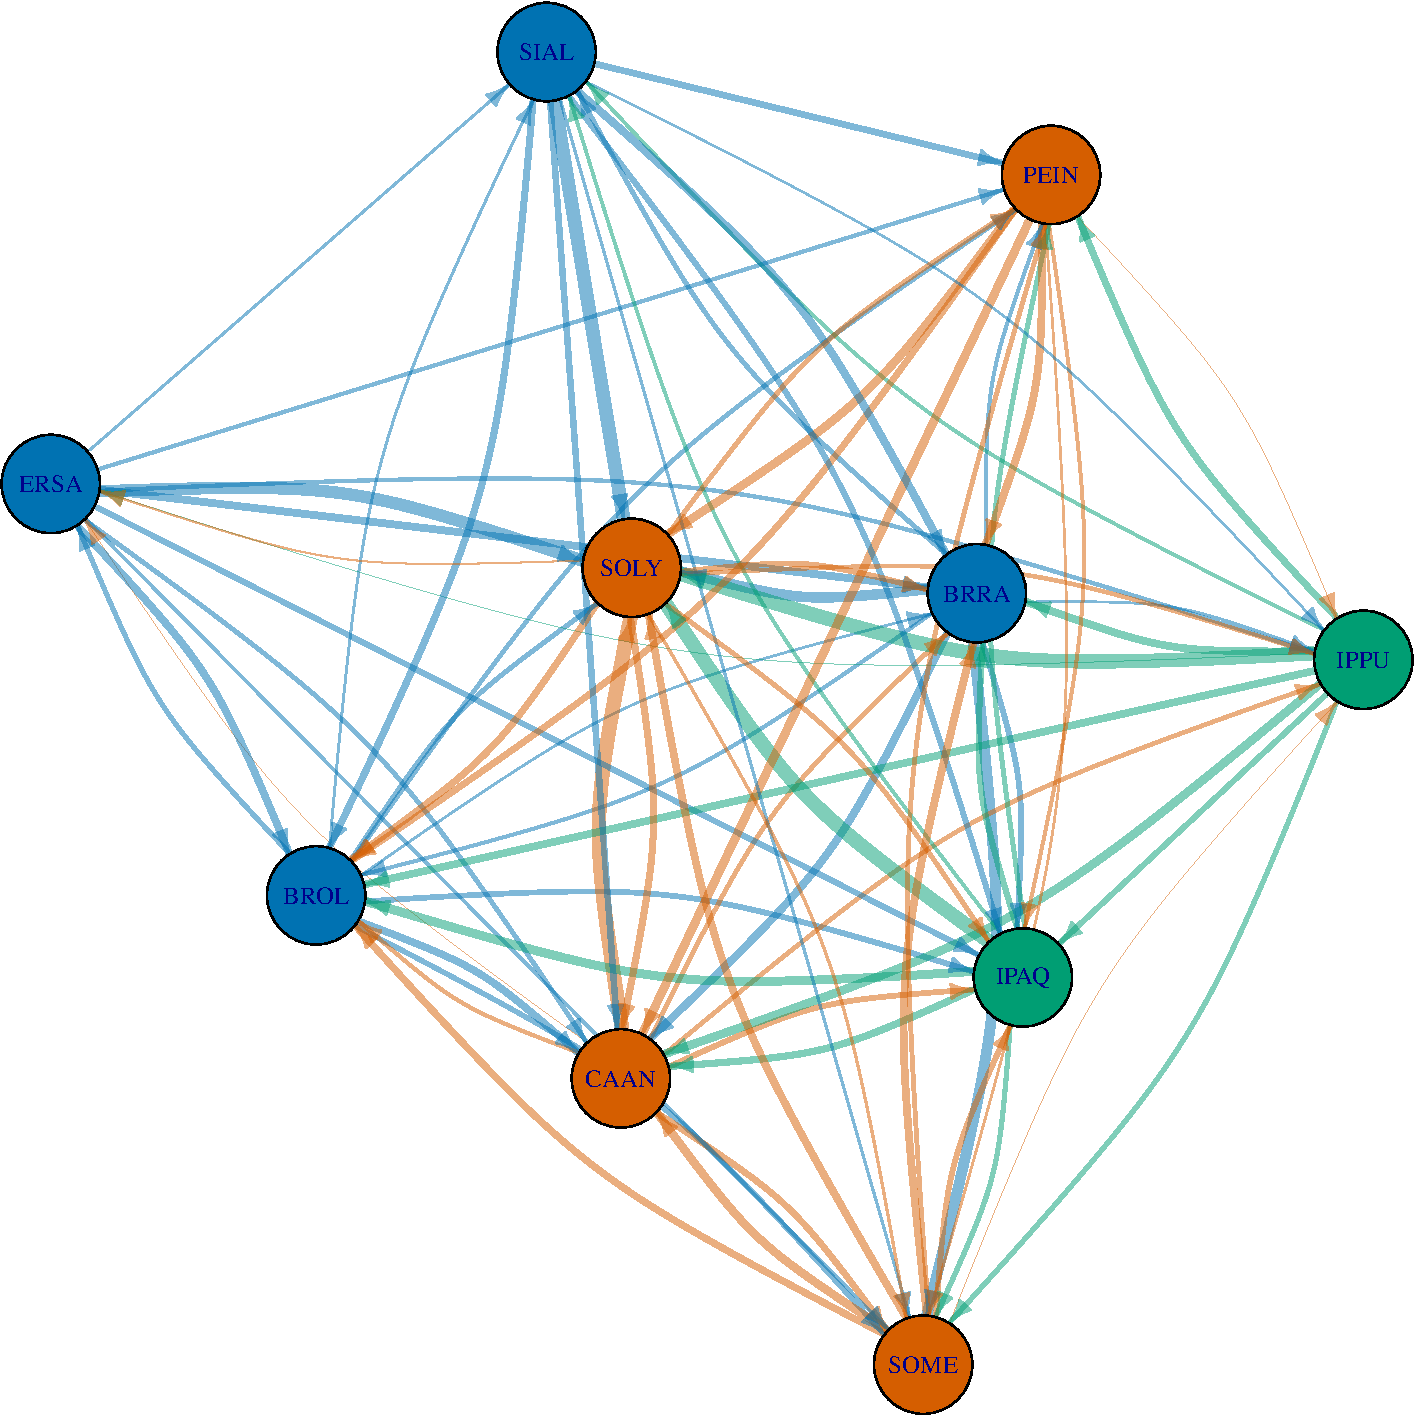
\includegraphics{Supp_Material_files/figure-latex/unnamed-chunk-15-1.pdf}
\caption{\textbf{Fig. S7} Violin plot of the proportion of seeds
coverted to ovule (\%) for all species with four different
hand-pollination treatments: apomixis (orange), hand cross pollination
(green), hand self pollination (blue) and spontaneous selfing (yellow).
The coloured dots, represent the different values of seed set for each
treatment.}
\end{figure}

\newpage

\begin{figure}
\centering
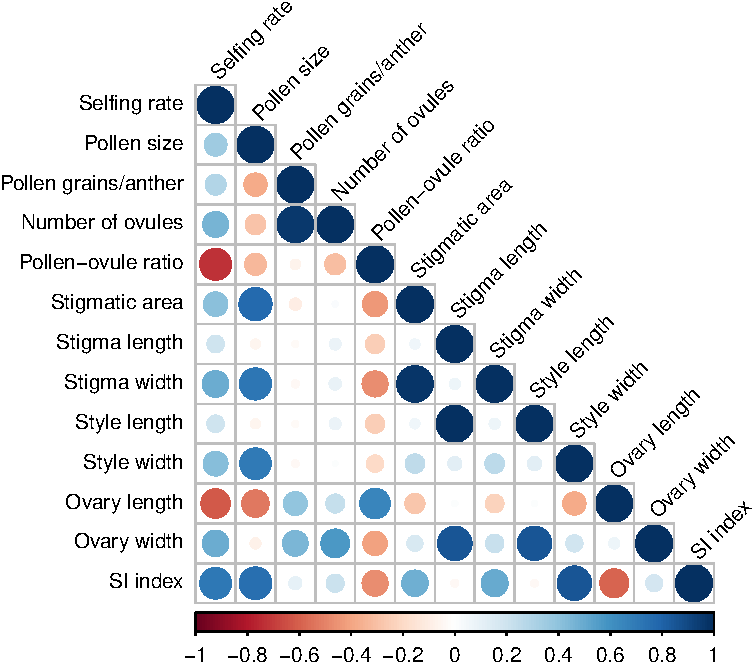
\includegraphics{Supp_Material_files/figure-latex/unnamed-chunk-16-1.pdf}
\caption{\textbf{Fig. S8} Grouped effect sizes (95\% confidence
intervals) of the different families on each focal species. For each
species, the grouped effect by family is compared with the control
treatment of hand cross pollination with conspecific pollen. The control
treatment is represented in yellow and vertically intersected with a
dashed line through the mean effect size in order to help the visual
interpretation of the effect sizes. Any value to the left of the
vertical dashed line represents a negative impact of foreign pollen. The
different effect sizes and confidence intervals are coloured by family:
Solanaceae (orange), Brassicaceae (blue) and Convolvulaceae (green).}
\end{figure}

\end{document}
